\section{Introduction}
\label{sec:introduction}

% state the learning objective 
The objective of this laboratory assignment is to study a circuit with resistances, sinusoidal voltage source and a capacitor (Fig.1). The main objective is to simulate the circuit using NGspice and compare results with the theoretical analysis. \par

\begin{figure}[H] \centering
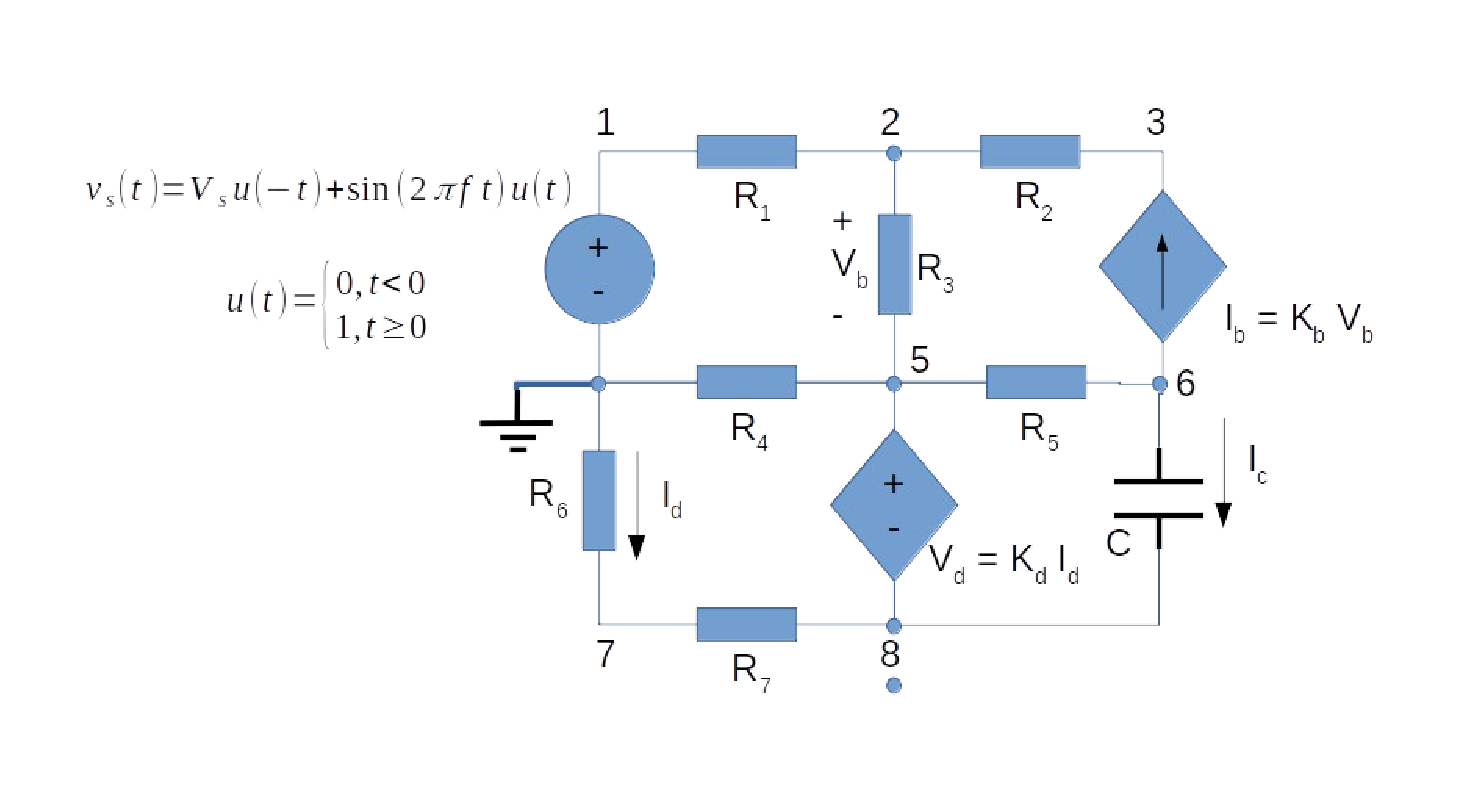
\includegraphics[width=0.6\linewidth]{circuito.pdf}
\caption{T2's given circuit.}
\label{fig:circuito}
\end{figure}

Firstly, in the theoretical analysis we will determine the voltages in all nodes and the currents in all branches using the nodal method, like in the previous laboratory assignment. Then, we calculate the equivalent resistance ($R_{eq}$) as seen from the capacitor terminals and determined the natural solution for $V_{6n}(t)$ and plot the result from 0ms to 20ms. The forced solution was also obtainned in the same interval (for f=1KHz) and the total solution was plotted for -5ms to 20ms. At last, the frequency response was calculated and the results were analised. \par
At the same time, the circuit was simulated using NGspice in order to obtain the same results and, considering that some of them could be lightly different, they were compared and analised.\par
The data used was the following:
\begin{center}
  \begin{tabular}{ | c | c | }
    \hline    
    {\bf Name} & {\bf Value [F, V, $\Omega$ or S]} \\ \hline
    $R_1$ & 1.04765357286e3 \\ \hline 
    $R_2$ & 2.06140068334e3 \\ \hline 
    $R_3$ & 3.03459085363e3 \\ \hline 
    $R_4$ & 4.00398818216e3 \\ \hline 
    $R_5$ & 3.11499853456e3 \\ \hline 
    $R_6$ & 2.04588646991e3 \\ \hline 
    $R_7$ & 1.04390152967e3 \\ \hline 
    $V_s$ & 5.02522591213 \\ \hline 
    $C$ & 1.00982536324e-6 \\ \hline
    $K_b$ & 7.28209304852e-3 \\ \hline
    $K_c$ & 8.36641247715e3 \\ 
    \hline
  \end{tabular}
\end{center}



